\chapter{Raft Algorithm}
\section{About Raft Algorithm}
\hspace{10mm} Raft is a consensus algorithm that was primarily designed to be easier
to understand and to work with than Paxos. Applying a communication model
whereby nodes converse and hold a copy of transactions, it facilitates the process
of electing a leader and reaching consensus over the network state. The Raft
system was devised by Diego Ongaro and John Ousterhout in 2013, and Now many use
it nowadays. It employs this protocol within a distributed system in order to
ensure that all the nodes in that distributed system agree regarding the state
of the network.
\newline

\section{States in Raft Algorithm}
The Raft algorithm consists of three main roles: leaders, followers, and candidates.
\begin{itemize}
    \item \textbf{Leaders:} They manage the replication of the log and actually
        coordinate the consensus process. They send heartbeat messages to the followers
        which maintains their authority and lets them know that indeed the network
        is in sync.

    \item \textbf{Followers:} Followers are nodes that listen to the leader and
        replicate the log. Respond to requests from the leader and other followers
        to maintain consistency in the network.

    \item \textbf{Candidates:} Candidates are nodes which are running for
        election as the leader. They send request votes to other nodes in the network
        to become the leader. If a candidate wins votes from a simple majority
        of the nodes, then that candidate becomes the leader of the distributed system.
\end{itemize}

\section{Terms in Raft Algorithm}
Raft divides time into terms of arbitrary length, numbered with consecutive
integers. Each term begins with an election, during which one or more candidates
attempt to become a leader. When a candidate receives votes from the majority of
nodes, it is considered to be a network leader for that term. If a leader fails or
behaves inappropriately, a new term is It thus starts, and a new leader is elected.
\newline

\section{Phases in Raft Algorithm}
The Raft algorithm works in two main phases: leader election and log replication.
\begin{itemize}
    \item Leader Election: In the leader election phase, nodes in the network compete
        to become the leader. If a node does not hear from the leader for a
        certain period of time, it becomes a candidate and requests votes from other
        nodes. If a candidate receives votes from a majority of nodes, it becomes
        the leader. Followers accept the leader if it has the most up-to-date
        log. Each term begins with a leader election, and a new leader is
        elected if the current leader fails or behaves incorrectly.

    \item Log Replication: Once a leader is elected, it sends heartbeat messages
        to followers to maintain its authority. The leader receives requests
        from clients and appends them to its log. It then replicates the log to followers,
        who apply the changes to their own logs to maintain consistency.
\end{itemize}
Raft ensures that the network remains available and consistent even if some nodes
fail or behave incorrectly.
\begin{center}
    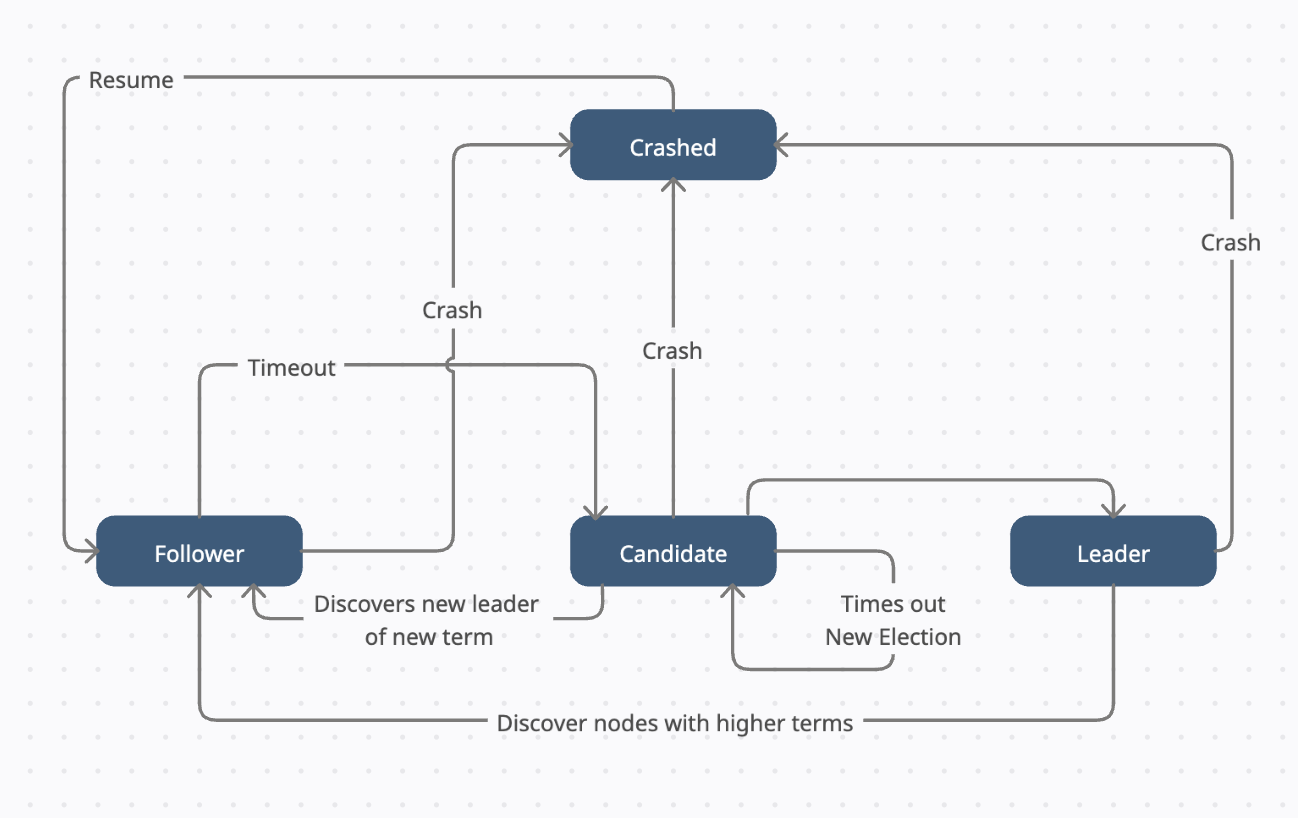
\includegraphics[width=145mm]{./Images/StatesAndTransitions.png}
\end{center}

\section{Log Replication in Raft Algorithm}

After electing a leader, it starts processing client requests. When a client
wants to update the log, the leader first updates its version of log entry in local
memory. Then sends this updated entry to every follower. Every follower checks the
new entry against its log in order to make sure that this new entry does not conflict
with the existing ones in the log. When no conflicts occur, the follower updates
its log and reports back to the leader. Once the leader gets acknowledgments
from a majority of followers, it considers the entry "committed" and writes it in
its state machine. The leader then notifies both the followers and the client
that the entry is committed. Upon getting this message, followers also log the
entry in their own state machine writing that it is "committed." Once committed,
the log entry becomes durable and cannot be rolled back.
\section{Safety in Raft Algorithm}

Raft ensures safety by enforcing rules on both the leader election process and
log replication. For leader election,

% Start list
\begin{itemize}
    \item A candidate can only be elected as leader if it receives votes from a majority
        of nodes. This ensures that the leader has the support of the majority
        of the network and prevents multiple leaders from being elected in the
        same term.

    \item Followers only vote for candidates whose logs are at least as up-to-date
        as their own. This ensures that the leader has the most recent log and
        prevents outdated entries from being committed.

    \item A candidate's log is considered more up-to-date if its last entry has a
        higher term, or if it has a longer log length for the same term. For log
        replication, the leader commits only those log entries that belong to
        its current term. However, entries from previous terms can be considered
        committed if they are followed by entries from the current term. This ensures
        that incorrect or outdated entries are not permanently applied,
        maintaining the system's integrity.
\end{itemize}

% Raft Roles and State Transitions
\section{Raft Server Roles and State Transitions}

Each server in Raft can be in one of three states: Follower, Candidate Leader or
Crashed.
\begin{itemize}
    \item \textbf{Follower:} Passive role; responds to requests from leaders and
        candidates.

    \item \textbf{Candidate:} Active role; tries to become the leader by starting
        an election.

    \item \textbf{Leader:} Active role; manages the log replication process and handles
        client requests.

    \item \textbf{Crashed:} A server that is not currently running, or has failed.
\end{itemize}

The state transitions among these roles occur based on timeouts, election
results, and message exchanges.
\subsection{Follower}

\textbf{Initial State:} When the system starts, each server begins as a follower.
\newline
\textbf{Actions:}
\begin{itemize}
    \item It Follows the leader.

    \item Responds to requests from the leader.

    \item If no messages from the leader or candidates are received within a specific
        election timeout, the follower becomes a candidate.
\end{itemize}

\textbf{State Transitions:}

\begin{itemize}
    \item \textbf{Follower → Candidate}: If the election timeout expires without
        hearing from a leader.

    \item \textbf{Follower → Follower}: If it receives an AppendEntries (heartbeat)
        from a valid leader.

    \item \textbf{Follower → Follower}: If it receives a RequestVote RPC with a higher
        term than its own, it updates its term and remains a follower.

    \item \textbf{Follower → Follower}: If it receives a RequestVote RPC with a lower
        term than its own, it ignores the request.

    \item \textbf{Follower → Crashed}: If the server crashes or is shut down(Maybe
        due to network failure).
\end{itemize}

\subsection{Candidate}
\textbf{Conditions to become Candidate:} If a follower does not receive any
messages (like AppendEntries) from a leader within an election timeout.
\newline
\textbf{Actions:}
\begin{itemize}
    \item Increments its current term.(Term is basically a counter that
        increases with each new election.)

    \item Votes for itself.

    \item Sends RequestVote RPCs to other servers.

    \item Waits to receive votes from a majority of servers.

    \item If it wins the election (majority votes), it becomes the leader.

    \item If another server claims a higher term, it steps down to follower.

    \item If the election timeout elapses without winning, it starts a new
        election.
\end{itemize}

\textbf{State Transitions:}
\begin{itemize}
    \item \textbf{Candidate → Leader}: If it receives votes from a majority of the
        servers.

    \item \textbf{Candidate → Follower}: If it receives an AppendEntries from a valid
        leader (with a higher or equal term).

    \item \textbf{Candidate → Candidate}: If the election timeout elapses without
        a majority, it restarts the election with an incremented term.

    \item \textbf{Candidate → Crashed}: If the server crashes or is shut down(Maybe
        due to network failure).
\end{itemize}

\subsection{Leader}
\textbf{Conditions to become Leader:} When a candidate wins the election.
\newline
\textbf{Actions:}
\begin{itemize}
    \item Sends periodic AppendEntries (heartbeat) messages to all followers to maintain
        authority.

    \item Responds to client requests by appending entries to its log and replicating
        these to followers.

    \item If an entry is committed (a majority of followers have appended it),
        it applies the entry to its state machine.

    \item If the leader crashes, followers will not receive heartbeats and will
        start a new election.
\end{itemize}

\textbf{State Transitions:}
\begin{itemize}
    \item \textbf{Leader → Follower}: If it discovers a server with a higher term
        (in AppendEntries or RequestVote RPC).

    \item \textbf{Leader → Leader}: As long as it has authority (sends
        heartbeats) and there is no term conflict.

    \item \textbf{Leader → Crashed}: If the server crashes or is shut down(Maybe
        due to network failure).
\end{itemize}

\subsection{Crashed}
\textbf{Conditions to become Crashed:} When a server crashes or is shut down(Maybe
due to network failure).
\newline
\textbf{Actions:}
\begin{itemize}
    \item Does not participate in the election process.

    \item Does not respond to messages from other servers.

    \item When it restarts, it reverts to a follower and updates its term.
\end{itemize}

\textbf{State Transitions:}
\begin{itemize}
    \item \textbf{Crashed → Follower}: When the server restarts, it reverts to a
        follower and updates its term.
\end{itemize}

\section{Process}

% \Start number list
\begin{enumerate}
    \item \textbf{Start:}
        \begin{itemize}
            \item All servers start as followers, waiting for a leader to be
                appointed.
        \end{itemize}

    \item \textbf{Election Trigger:}
        \begin{itemize}
            \item If a follower does not receive any messages from a leader within
                a specific election timeout, it becomes a candidate and starts
                an election.
        \end{itemize}

    \item \textbf{Election Process:}
        \begin{itemize}
            \item Each candidate increases its term, votes for itself, and sends
                RequestVote messages to other servers.

            \item If a candidate receives votes from a majority (in this case, 2
                out of 3 servers), it becomes the leader.

            \item If another server claims a higher term or another candidate receives
                a majority of votes, it reverts to follower or retries the
                election after another timeout.
        \end{itemize}

    \item \textbf{Leader Operations:}
        \begin{itemize}
            \item The elected leader starts sending heartbeats (AppendEntries
                with no data) to maintain its leadership.

            \item When a client request is received, the leader appends the
                request to its log and sends AppendEntries to followers to
                replicate the log.

            \item Once a majority of followers confirm the log entry, it’s
                marked as committed, and the leader can apply it to its state machine.
        \end{itemize}

    \item \textbf{Handling Failures:}
        \begin{itemize}
            \item If a leader crashes, followers will stop receiving heartbeats
                and transition to candidates after an election timeout.

            \item They start a new election, and a new leader is chosen.
        \end{itemize}

    \item \textbf{Handling Network Partitions:}
        \begin{itemize}
            \item If the network partition divides the servers such that a minority
                partition cannot form a quorum, servers in that partition will
                remain followers or candidates.

            \item When the network partition heals, servers with outdated terms
                will revert to followers after receiving messages from the
                current leader.
        \end{itemize}
\end{enumerate}